\subsubsection{Python}

\begin{wrapfigure}{r}{0.25\textwidth}
  \begin{center}
    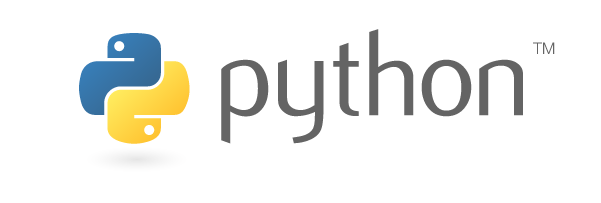
\includegraphics[width=0.2\textwidth]{python}
  \end{center}
\end{wrapfigure}
Jako język programowania wybraliśmy język \textbf{Python}.

\textbf{Python} to interpretowany język ogólnego zastosowania, pozwalający programować na wysokim poziomie abstrakcji.
Język oparty jest na wielu paradygmatach programowania: programowaniu obiektowym, programowaniu funkcjonalnym i programowaniu imperatywnym.
Typowanie w \textbf{Pythonie} jest dynamiczne, a typy są mocne.
Zarządzanie pamięcią odbywa się dynamicznie.

Interpretery \textbf{Pythona} dostępne są na wszystkie popularne systemy operacyjne, wiele z nich jest otwartym oprogramowaniem.
Sama specyfikacja języka zarządzana jest przez \emph{Python Software Foundation}~--- niezależną organizację non-profit.

Głównym powodem, dla którego zdecydowaliśmy się na język \textbf{Python} to jego popularność.
Język ten ma opinię języka o bardzo dobrej dokumentacji.
Popularność wpływa także na dostępność dużej ilości otwartych bibliotek, z których wiele jest dojrzałych i wysokiej jakości.

Wielu z nas korzysta na codzień z systemu GNU/Linux, gdzie wiele aplikacji jest napisanych w języku \textbf{Python}.
Znajomość języka \textbf{Python} pozwoliłaby nam więc robić zmiany w aplikacjach, z których korzystamy na codzień.

Jednym z powodów, dla którego wybraliśmy język \textbf{Python} był także fakt, że nikt z nas go nie znał.
Wybranie nieznanego dotąd języka miało sprawić, że projekt będzie bardziej interesujący oraz zwiększyć kompetencje zawodowe członków zespołu
\footnote{W razie gdyby projekt nie okazał się hitem na miarę Napstera i musielibyśmy się jeszcze kiedykolwiek starać o pracę.}
.

\subsection{pyparsing}
\textbf{Pyparsing} to jedna z bibliotek, które skłoniły nas do wybrania języka \textbf{Python} do realizacji tego projektu.

Biblioteka pozwala w prosty sposób zbudować rekursywny parser zstępujący.
Gramatyka, która ma być parsowana, określana jest za pomocą języka \textbf{Python} w plikach źródłowych projektu (W naszym przypadku w pliku \texttt{lexer.py}).
Pyparsing jest używany w takich projektach jak Django, pydot czy Graphite.

Parsowaną gramatykę opisuje się tworząc odpowiednie obiekty.
Obiekty te mogą reprezentować symbole terminalne (wyrażenia regularne, zestawy znaków, pojedyńcze znaki lub ich ciągi) lub ich produkcje.
Każdemu obiektowi można przypisać akcję, która zostanie wykonana, gdy dany symbol zostanie wczytany.
